\documentclass[/Users/ikedahajime/GitHub/reserch/master_report/thesis]{subfiles}
% このファイル内だけのコマンド
\begin{document}
\renewcommand{\prechaptername}{付録}
\renewcommand{\postchaptername}{}
\renewcommand{\thechapter}{\Alph{chapter}}
\setcounter{chapter}{0}

% \chapter{予備研究の結果}
\chapter{壁の形状による影響}\label{subsec:result_abp_twowall}
2つの円を繋げて、それらの円における渦が同じ方向に回る(強磁性的)か反対の方向に回る(反強磁性的)か
を調べた研究が存在する\cite{beppuGeometrydrivenCollectiveOrdering2017}。この研究では、強磁性、反強磁性を
分ける要素は2つの円の間の距離であることがわかっている。この章では自己駆動力がこの現象に与える
影響を明らかにするため、ABPについてのシミュレーションを行う。%TODO:言い回し


シミュレーションにはABPを用い、ポテンシャルには WCA ポテンシャルを用いた。
壁は\figref{fig:wall_twowall}のようにおき、壁との相互作用についても同様に WCA ポテンシャルを用いた。
$r_{wall}$は$\bm{r}_{c_i}$を各粒子が存在する円の中心をさすベクトルとして$r_{wall}=R+0.5\sigma-\left|\bm{r}-\bm{r}_{c_i}\right|$
と表される。2つの円の接合部である$-0.5\sigma<x<0.5\sigma$においては仮想粒子を$(x,y)=(0,\pm\sqrt{(R+0.5\sigma)^2-(\Delta/2)^2})$
に置いて、それらとの相互作用を壁との相互作用とした。$\varphi=0.7、M=0.1$として、2つの円間の距離$\Delta$、
$Pe$をコントロールパラメータとした。
\begin{figure}
    \centering
    \begin{tabular}{c}
        \begin{minipage}{0.4\hsize}
            % \text{(b)}
            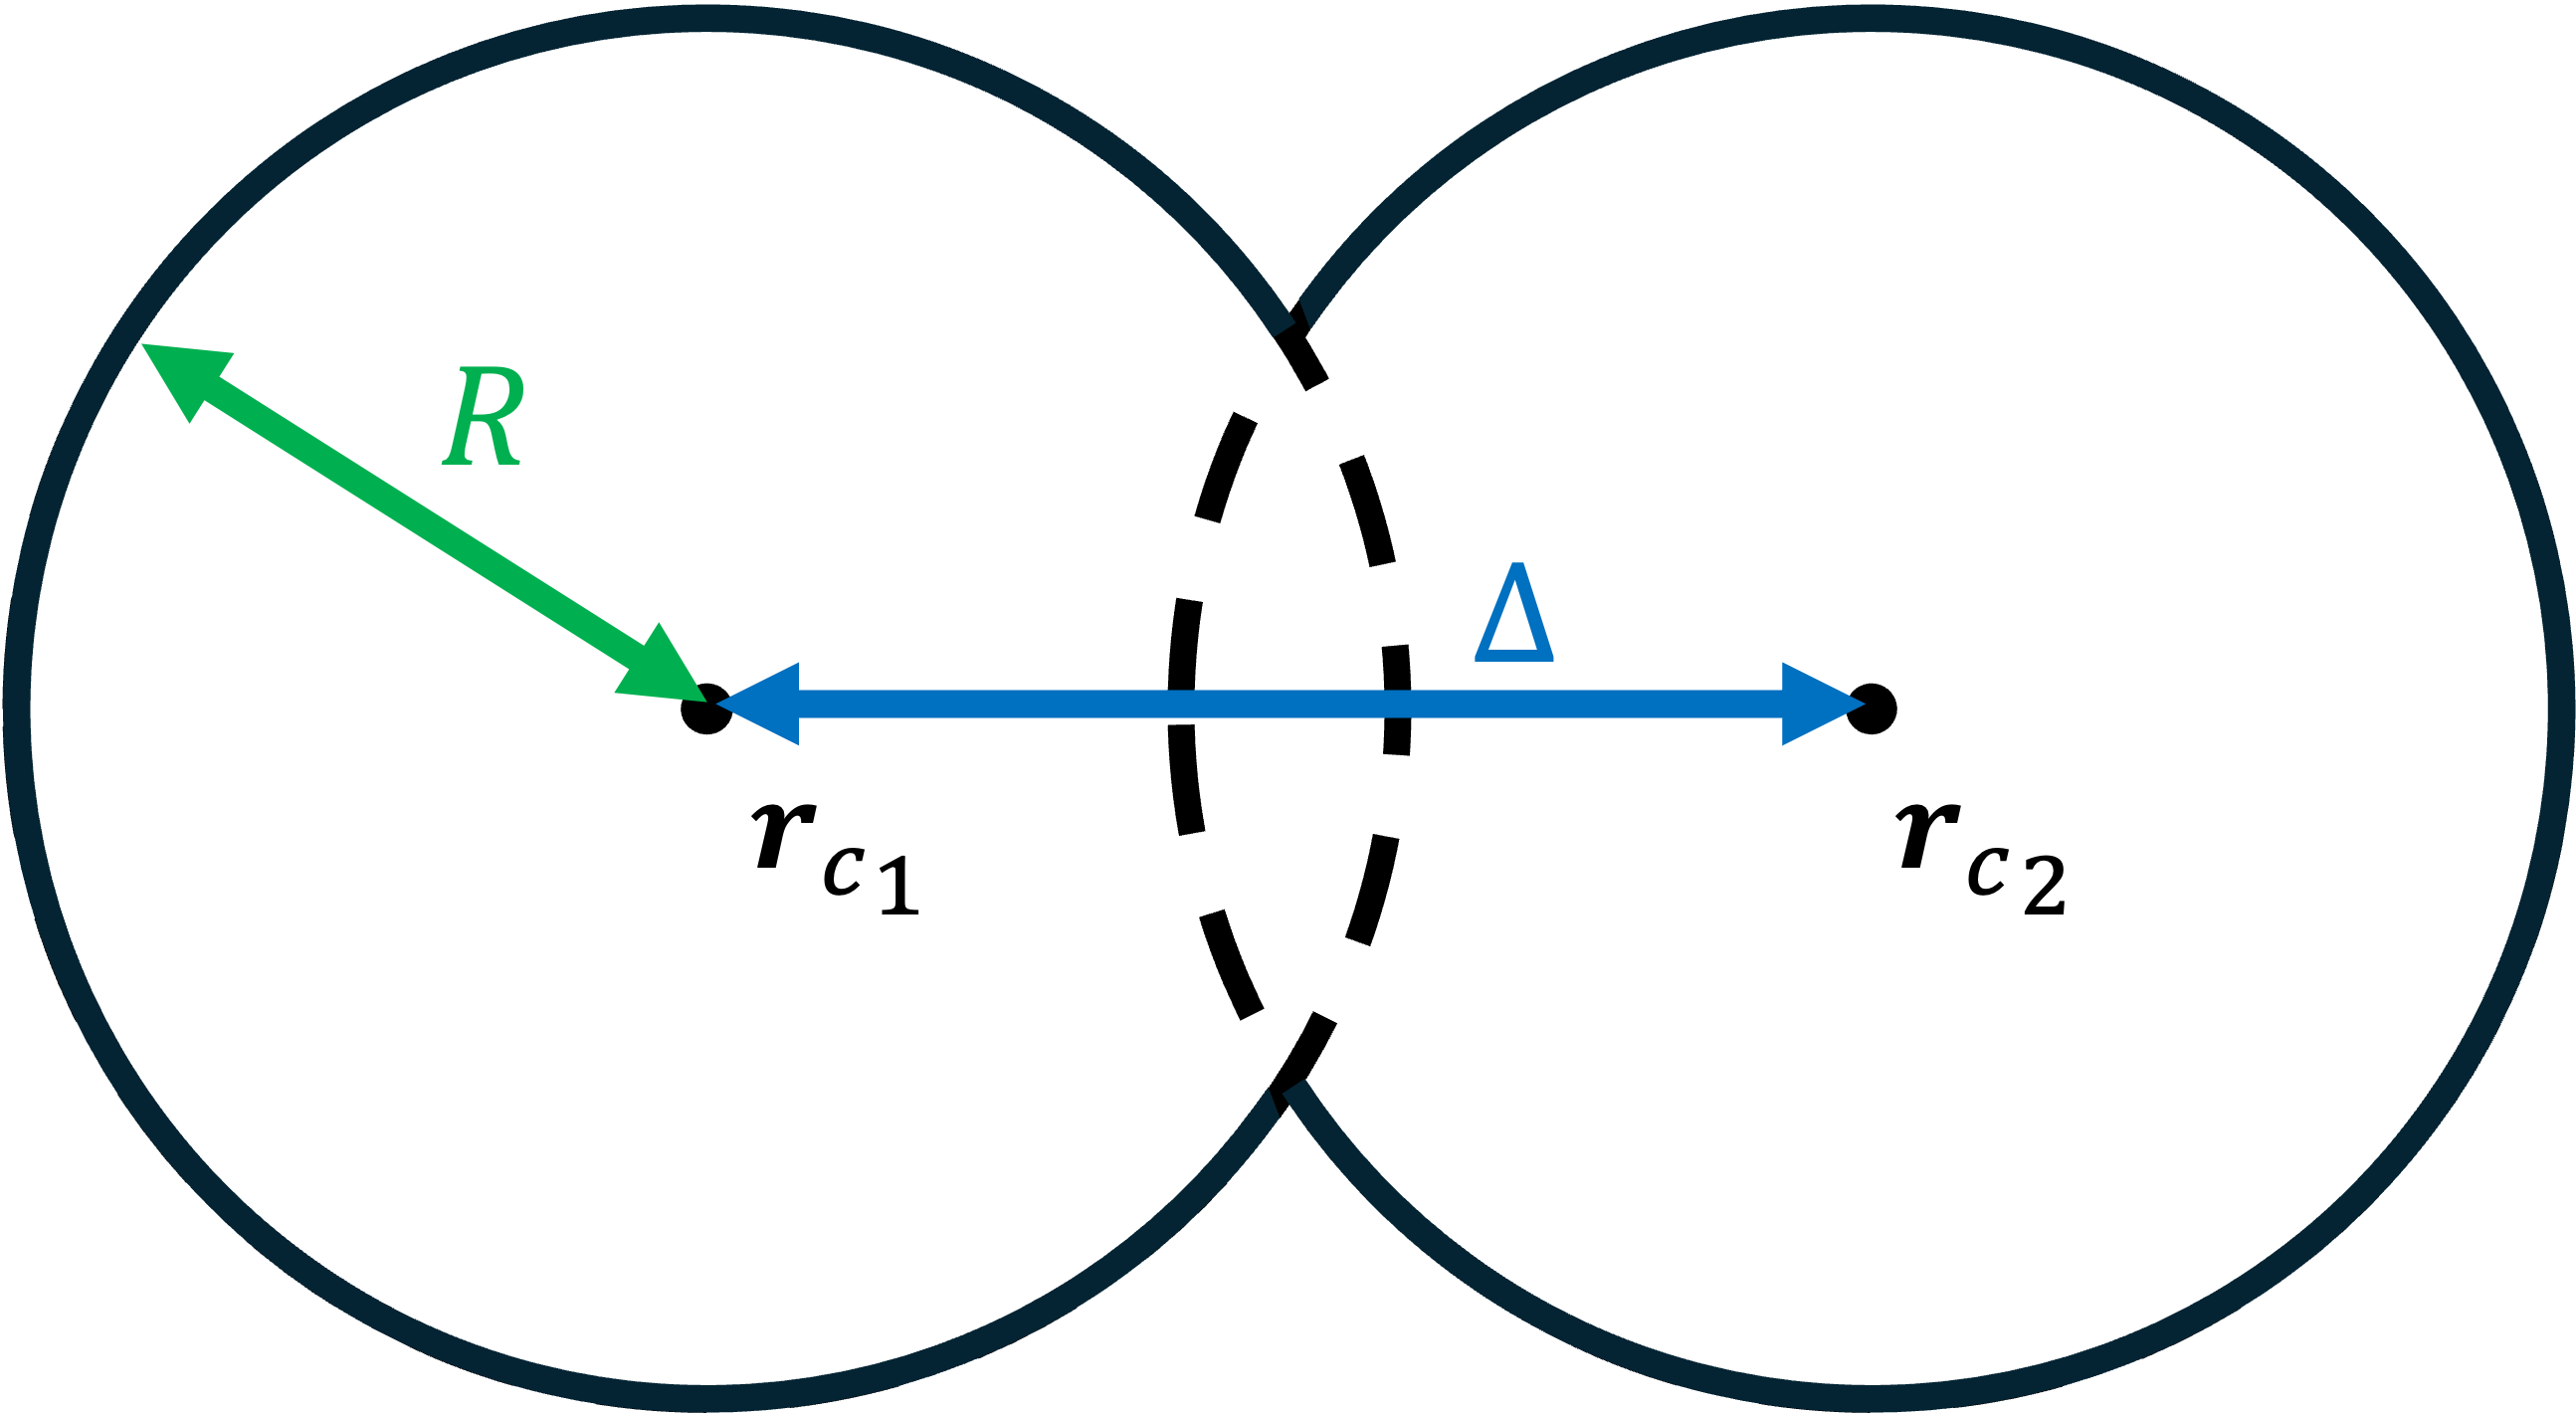
\includegraphics[width=\textwidth]{img/method/fig_twocer.png}
        \end{minipage}
    \end{tabular}
    \caption[Four sample images]
    {
        2つの円を繋げた場合の壁の模式図
    }
    \label{fig:wall_twowall}
\end{figure}

2つの円における渦の強磁性、反強磁性を判別するため、以下のオーダーパラメータを導入する。
\begin{equation}
    V_2={\mathop{\mathrm{sign}}\nolimits} (V)\sqrt{|V|}
\end{equation}
ここで、$V=(\sum_{x<0} L_{zc_1}/|L_{zc_1}|)(\sum_{x>0}L_{zc_2}/|L_{zc_2}|)$で、$L_{zc_i}$は$r_{c_i}$を中心とする角運動量である。
このパラメータは、渦が強磁性的であれば1、反反共自制的であれば-1にそれぞれ近づくことを表す。
また、この系における渦秩序変数を以下のように定義する。
\begin{equation}
    \varphi_2=\frac{(\sum_{x<0} \left|\bm{v}\cdot \bm{t}_{1} \right|+\sum_{x>0} \left|\bm{v}\cdot \bm{t}_{2} \right|)/\sum_i v_i -2/\pi}{1-2/\pi}
\end{equation}
ここで、$\bm{t}_1、\bm{t}_2$は、それぞれ左、右の円における壁に並行な単位ベクトル。


その結果は\figref{fig:twocer_lo0.7_r10_m0.1}の通りである。
半径$R=10$、$\varphi=0.7、M=0.1$のパラメータを用いた。

\begin{figure}
    \centering
    \begin{tabular}{c}
        \begin{minipage}{0.4\hsize}
            \text{(a)}
            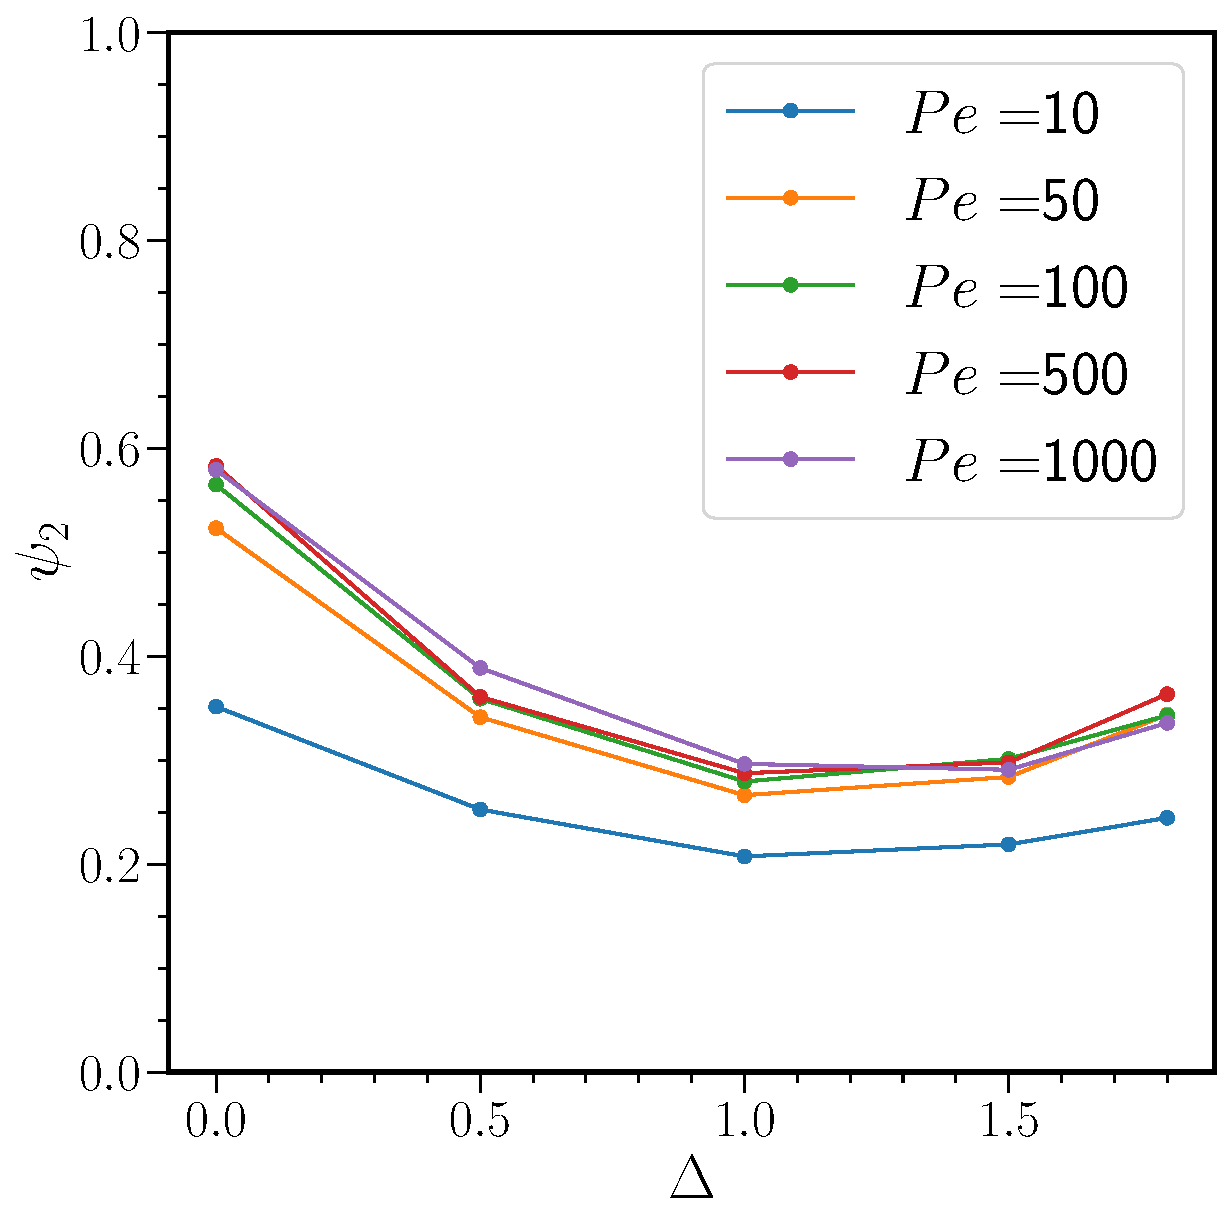
\includegraphics[width=\textwidth]{img/bit/ani_test/psi_20.70.110.pdf}
        \end{minipage}
        % \begin{minipage}{0.3\hsize}
        %     \text{(b)}
        %     \includegraphics[width=\textwidth]{img/bit/ani_test/L_{z2}0.70.110.pdf}
        % \end{minipage}
        \begin{minipage}{0.4\hsize}
            \text{(b)}
            \includegraphics[width=\textwidth]{img/bit/ani_test/V_{2}0.70.110.pdf}
        \end{minipage}
    \end{tabular}
    \caption[two_hdlm]
    {
        $\varphi=0.7、R=10、M=0.1$における(a)$\varphi_2$、(b)$V_2$のグラフ。
        横軸は2つの円の間の距離である。
    }
    \label{fig:twocer_lo0.7_r10_m0.1}
\end{figure}
まず$Pe$依存性について見ると、$\varphi_2、V_2$においてそれらの絶対値が大きくなっており、円が1つの場合
と同様に$Pe$が大きくなると粒子が同じ方向へと流れることがわかる。
次に$\Delta$依存性について見ると、$\Delta\simeq1.4$周りで$V_2$の符号が正から負へと変化しており、
これは$\Delta$を大きくすると2つの円の流れが同じ方向から逆の流れへと変化することを表す。
\end{document}
